\documentclass[11pt]{article}

\usepackage{graphicx}
\usepackage{framed}
\usepackage{hyperref}

\marginparwidth 0.5in 
\oddsidemargin 0.25in 
\evensidemargin 0.25in 
\marginparsep 0.25in
\topmargin 0.25in 
\textwidth 6in \textheight 8 in

\begin{document}
\hfill\vbox{\hbox{Jude Shin, Torrey Zachs}
		\hbox{CSC 321, Section 07}	
		\hbox{Module 2: Block Ciphers}	
		\hbox{\today}}\par

\bigskip
\centerline{\Large\bf Lab 02: Symmetric Key Cryptography Exploration}\par
\bigskip

This lab explores symmetric key cryptography security with both Electronic Codebook (ECB) and Cipher Block Chaining (CBC) modes. This lab also demonstrates the limits and exploitations of each, as well as a performance study of public versus symmetric key algorithms. This lab was completed using {\tt Python} and {\tt PyCryptodome}. All the code can be found in our remote \href{https://github.com/jude-shin/CSC\_321}{GitHub} repository.

% ============================================================================
\section*{Environment}

If you want to run and test the code, a virtual environment should first be set up with the correct requirements. This ensures that there is consistency between all of the packages used within this project.

\begin{itemize}
	\item Make a virtual environment (venv) with Python.

		\verb|$ python3 -m venv .venv|

	\item Activate the venv.

		\verb|$ source .venv/bin/activate|

	\item Install the requirements using pip.

		\verb|$ pip install -r requirements.txt|

	\item Whenever you are done, you can deactivate the venv.

		\verb|$ deactivate|

\end{itemize}

% ============================================================================
\section*{Task 1: Modes of Operation}
\subsection*{Abstract}
The main data type used was the \verb|bytes| data type, which could be treated as a fixed array of bytes; this data type could be iterated over and indexed, making it easy to locate particular parts of an encrypted or decrypted message. The path to the BMP that the user wants to encrypt is listed as the first command line argument. Both methods of single-key encryption use ``blocks'' of data. In our case, we chose to use 128-bit (16-byte) chunk sizes. In our example, we will encrypt some BMP images. In both cases, the first 54 bytes were removed as they were the BMP headers. Then the rest of the data was padded to be divisible by the chosen block size.

\subsection*{Code Breakdown}
\subsubsection*{task1.py}

The Python script \verb|task1.py| executes two functions, one to encrypt a file with ECB, and one to encrypt a file with CBC. 

\begin{framed}
\begin{verbatim}
if __name__ == '__main__':
    if len(sys.argv) == 2:
        plaintext_file: str = sys.argv[1]

        encrypt_bmp_with_ecb(plaintext_file)
        encrypt_bmp_with_cbc(plaintext_file)

    else:
        print('One cmd line arg required!')
\end{verbatim}
\end{framed}

\subsubsection*{ECB Code}

The \verb|encrypt_bmp_with_ecb| function will take a file path for the BMP file and then open it in bytes. It will then generate a random key; note that this has to be random bytes of the same length as the BLOCK\_SIZE. The data is also padded to the BLOCK\_SIZE. An AES object is used, but the encryption is done only in BLOCK\_SIZEs. We could have used the defined \verb|.encrypt()| functions for this, but for this lab we are choosing to implement the blocks ourselves in order to highlight the differences between ECB and CBC methods. Each block that is encrypted is subsequently added to the \verb|encrypted_text| variable. Finally, the BMP header is prepended to the encrypted data. The encrypted data is then written to a new file. For testing purposes, the key is also written to a separate file. 

The \verb|decrypt\_ecb| function was implemented with the package's \verb|.decrypt()| function in order to verify that our custom encrypt function was working as intended.

\begin{framed}
\begin{verbatim}
HEADER_SIZE: int = 54
BLOCK_SIZE: int = 16

def encrypt_ecb(text: bytes, key: bytes) -> bytes:
    cipher = AES.new(key=key, mode=AES.MODE_ECB)

    encrypted_text: bytes = b''
    for i in range(0, len(text), BLOCK_SIZE):
        chunk: bytes = text[i:i+BLOCK_SIZE]
        encrypted_text = encrypted_text + cipher.encrypt(chunk)
    return encrypted_text 

def decrypt_ecb(text: bytes, key: bytes) -> bytes:
    # Cipher Function
    cipher = AES.new(key=key, mode=AES.MODE_ECB)
    
    # We can use this library
    return cipher.decrypt(text)

def verify_ecb_encryption(text: bytes, encrypted_text: bytes, key: bytes):
    decrypted_text = decrypt_ecb(encrypted_text, key)
    if (text == decrypted_text):
        print("ecb encryption Verified")
    else:
        print("ecb decrypted value did not match original plain text")

def encrypt_bmp_with_ecb(plaintext_file: str):
    text: bytes | None = read_bytes(plaintext_file)

    key: bytes = random.randbytes(BLOCK_SIZE)
    print(f'key: {key}')
    header: bytes = text[:HEADER_SIZE]
    data: bytes = text[HEADER_SIZE:]
    padded_data: bytes = add_padding(data, BLOCK_SIZE)

    encrypted_text: bytes | None = encrypt_ecb(padded_data, key)
    verify_ecb_encryption(padded_data, encrypted_text, key);

    encrypted_text = header + encrypted_text

    bmp_name = plaintext_file.replace('assets/', '').replace('/', '') \
                             .replace('.bmp', '')
    dir_ = 'encryptions/ecb/'

    write_bytes(dir_ + 'encryption_of_' + bmp_name + '.bmp', encrypted_text)
    write_bytes(dir_ + 'key_of_' + bmp_name + '.txt', key)
\end{verbatim}
\end{framed}

\subsubsection*{CBC Code}

This is almost the same as ECB; however, the previous ciphertext block is first \verb|xor|ed with the current plaintext block before that block is put through the ECB encryption algorithm. This is where the custom implementation of \verb|/encrypt()| becomes more interesting. Before passing the plaintext block into the \verb|.encrypt()| function, we first \verb|xor| it with the previous ciphertext. As for the very first block (which has no ``previous'' ciphertext), a random initialization vector (IV) is used in its place. Processing the header and padding follows the same procedure as the ECB encryption. The encrypted file is written to a file. Again, for testing purposes, the key and IV are written to files as well.

When writing the custom \verb|.encrypt()| function for the CBC method, the AES.MODE had to be specified as \verb|AES.MODE_ECB|. If it were \verb|AES.MODE_CBC|, then an IV would automatically be applied every time \verb|.encrypt()| was called; however, CBC only applies the IV once at the beginning block.

\begin{framed}
\begin{verbatim}
HEADER_SIZE: int = 54
BLOCK_SIZE: int = 16

def encrypt_cbc(text: bytes, key: bytes, iv: bytes) -> bytes:
    # NOTE: if you specify ECB, then it will probably try to use
		# some input vector every time you call encrypt
    cipher = AES.new(key=key, mode=AES.MODE_ECB)

    encrypted_text: bytes = b''
    prev: bytes = iv
    for i in range(0, len(text), BLOCK_SIZE):
        chunk: bytes = text[i:i+BLOCK_SIZE]

        xor: bytes = xor_bytes(chunk, prev)

        prev = cipher.encrypt(xor) 

        encrypted_text = encrypted_text + prev

    return encrypted_text 

def decrypt_cbc(text: bytes, key: bytes, iv: bytes) -> bytes:
    # Cipher Function
    cipher = AES.new(key=key, mode=AES.MODE_CBC, iv=iv)
    
    # We can use this library
    return cipher.decrypt(text)

def verify_cbc_encryption(text: bytes, encrypted_text: bytes,
                          key: bytes, iv: bytes):
    decrypted_text = decrypt_cbc(encrypted_text, key, iv)
    if (text == decrypted_text):
       print("cbc encryption Verified")
    else:
        print("cbc decrypted value did not match original plain text")

def encrypt_bmp_with_cbc(plaintext_file: str) -> None:
    text: bytes | None = read_bytes(plaintext_file)

    # key must be BLOCK_SIZE bytes long (for AES-128)
    key: bytes = random.randbytes(BLOCK_SIZE)
    print(f'key: {key}')

    # iv  must be BLOCK_SIZE bytes long
    iv: bytes = random.randbytes(BLOCK_SIZE)
    print(f'iv: {iv}')
    
    header: bytes = text[:HEADER_SIZE]
    data: bytes = text[HEADER_SIZE:]
    padded_data: bytes = add_padding(data, BLOCK_SIZE)

    encrypted_text: bytes | None = encrypt_cbc(padded_data, key, iv)    
    verify_cbc_encryption(padded_data, encrypted_text, key, iv)

    encrypted_text = header + encrypted_text

    bmp_name = plaintext_file.replace('assets/', '').replace('/', '') \
                             .replace('.bmp', '')
    dir_ = 'encryptions/cbc/'

    write_bytes(dir_+'encryption_of_'+bmp_name+'.bmp', encrypted_text)

    write_bytes(dir_ + 'key_of_' + bmp_name + '.txt', key)
    write_bytes(dir_ + 'iv_of_' + bmp_name + '.txt', iv)
\end{verbatim}
\end{framed}

\subsubsection*{PKCS\#7 Code} 

The PKCS padding scheme adds a number of bytes to the end of the data, ensuring that the encryption algorithm has even blocks to work with. Let the number of remaining bytes that were filled be \verb|k|. Each byte that is appended to the end of the data is the integer \verb|k| represented as a byte. This, of course, is a well-defined padding system up to padding of 255 extra bytes.

\begin{framed}
\begin{verbatim}
# pad text bytes with pkcs#7 padding
def add_padding(text: bytes, block_size: int) -> bytes:
    # Get the remainder that is needed to become a multiple of block_size
    k: int = block_size - len(text)%block_size

    # k(byte) will be repeated k times
    single_byte: bytes = k.to_bytes(1, 'big')
    padding: bytes = single_byte * k

    # Append the padding to the end of the text 
    return text + padding 

# remove a padded text bytes with pkcs#7 padding
def strip_padding(text: bytes) -> bytes:
    # Read the last block (should be an int)
    k: int = text[-1]

    # If the number that are in the last k bytes does not match up
		# , then there was no padding (or a padding of 0)
    for i in range(k):
        if (k != text[-(i+1)]):
            return text 

    # Remove the last k bytes in text 
    return text[:-k]
\end{verbatim}
\end{framed}

\subsubsection*{Utilities Code}

Some helper functions were shared between the two encryption methods, like reading and writing bytes to a file. Note that we open the file with the binary mode (indicated by the 'b') to indicate that we want a \verb|bytes| data type instead of a file object.

\begin{framed}
\begin{verbatim}
def read_bytes(filename: str) -> bytes:
    with open(filename, 'rb') as f:
        return f.read()

def write_bytes(filename: str, text: bytes) -> None:
    with open(filename, 'wb+') as f:
        f.write(text)
\end{verbatim}
\end{framed}

\subsection*{Reproduction}

Running both encryption processes on a given BMP is as simple as activating the venv and then running \verb|task1.py| with the file to be encrypted.

\verb|(.venv) python task1.py ./path/to/image.bmp|

\subsection*{Results and Analysis}

The encrypted BMP images are included below. The ECB encryption (Figure \ref{fig:ecb}) presents a security flaw: patterns are noticeable and might reveal more information than was intended. Although this is the case, the benefit is that the algorithm is robust: it does not rely on previous steps of the encryption process. AES (Figure \ref{fig:cbc}) is shown to be more obscure because of the \verb|xor| on previous encrypted blocks, but this method allows errors in previous steps to propagate to the rest of the encryption.

\begin{figure}[!ht]
	\centering
	
\includegraphics[width=0.5\textwidth]{./assets/ecb_encrypted.jpg}
	\caption{A noticeable outline of the Cal Poly logo is shown.}
	\label{fig:ecb}
\end{figure}

\begin{figure}[!ht]
	\centering
	
\includegraphics[width=0.5\textwidth]{./assets/cbc_encrypted.jpg}
	\caption{No useful patterns are shown in this encrypted image.}
	\label{fig:cbc}
\end{figure}

% ============================================================================
\section*{Task 2: Limits of Confidentiality}
\subsection*{Abstract}

Bit (or byte) flipping is an exploit on block cipher encryption algorithms. Because we know that some of the plaintext is \verb|xor|ed with the previous ciphertext in CBC encryption, we can use a series of \verb|xor|s to flip bytes in a way that is somewhat predictable. In our example of this phenomenon, we took an arbitrary string and performed this bit-flipping attack to produce a desired string when decrypted.

\subsection*{Code Breakdown}

The substring that we chose to insert into our function was \verb|'ydmin=true'|. The target string was supposed to include the substring \verb|'addmin=true'| at the very end. Out of the whole concatenated string, the character \verb|'y'| happened to be located at the 21st position in the \verb|bytes| object. The method to byte-flip the targeted character involves \verb|xor|ing the target character (in our case 'a') with the plaintext character at that index (in our case 'y'). Finally, we must \verb|xor| that \verb|xor|ed byte one more time: with the byte of the ciphertext in the previous block (exactly BLOCK\_SIZE bytes away from the) index of the character of interest. Note that if we wanted to change a byte in the first block of the message, we would have to know the IV, as in CBC it acts as the ``previous'' block.

Once we have the newly \verb|xor|ed byte, we use it to replace the byte in the original encrypted message at the ``previous'' block's index.

Full Example: Suppose we have a message that is 16 bytes long. If each block was 8 bytes long, and the byte we wanted to manipulate was at position 10 (it is located at index 2 of the second block), the ``previous'' byte we would replace would be at index 2 of the original encrypted message.

When the decryption occurs, the bytes before will be scrambled and garbage; however, the block with the desired message will contain the new message with the manipulated byte.

\begin{framed}
\begin{verbatim}
if __name__ == '__main__':
    # The byte we want to flip is at position 21
    text: str = ';ydmin=true'
    mod_char: str = 'y'
    target_char: str = 'a'
    i: int = 21
    ti: int = i - BLOCK_SIZE

    encrypted_text = submit(text)
    decrypted_text = decrypt_cbc(encrypted_text, KEY, IV)

    xor: int = ord(mod_char) ^ ord(target_char)

    modified_byte: bytes = (encrypted_text[ti] ^ xor).to_bytes(1, 'big')
    modified_encrypted_text: bytes = encrypted_text[:ti] + (modified_byte) + encrypted_text[ti+1:]

    print(f'Verification result: {verify(modified_encrypted_text)}')
\end{verbatim}
\end{framed}

\subsubsection*{Submit Code}

This function simply took in a substring that we were going to manipulate (in our case, we chose \verb|'ydmin=true'|), added some extra text to the beginning and end, and then properly encrypted it with PKCS\#7 padding and CBC symmetric key encryption.

\begin{framed}
\begin{verbatim}
def submit(text: str) -> bytes:
    prepend: str = 'userid=456;userdata='
    append: str = ';session-id=31337'

    full_text: str = prepend + text + append 
    
    url_data: bytes = full_text.encode('utf-8')

    padded_url_data: bytes = add_padding(url_data, BLOCK_SIZE)
    encrypted_text: bytes = encrypt_cbc(padded_url_data, KEY, IV)

    return encrypted_text
\end{verbatim}
\end{framed}

\subsubsection*{Verify Code}

This function checked to see if our desired output string (in our case, we wanted to see \verb|';admin=true;'|) was in the decrypted message. The function took in a ciphertext (but in reality, the ciphertext was manipulated with the bit-flipping attack). It returns \verb|true| if the substring is present and \verb|false| if the substring is not present.

\begin{framed}
\begin{verbatim}
def verify(ciphertext: bytes) -> bool:
    search_str: str = ';admin=true;'

    # decrypt the string  
    decrypted_data: bytes = decrypt_cbc(ciphertext, KEY, IV)

    # In English please
    plain_str: str = parse.unquote(decrypted_data)

    return (search_str in plain_str)

\end{verbatim}
\end{framed}

\subsubsection*{Reproduction}

Running this test is as simple as activating the venv and then running \verb|task2.py|. The output should produce \verb|Verification result: true|, indicating that the bit-flipping attack was successful.

\verb|(.venv) python task2.py|

% ============================================================================
\section*{Task 3: Performance Comparison}
\subsection*{Abstract}

In this task we compare the performance of AES encryption with that of RSA encryption using the OpenSSL command: \$openssl speed <rsa/aes>. The \verb|openssl speed aes| benchmark gives a measurement of throughput directly in kb/sec. However, the \verb|openssl speed rsa| benchmark measures the speed at which four different RSA actions can be performed per second. These actions are: 1. sign/s, 2. verify/s, 3. encryptions/s, 4. decryptions/s. To compare the measurements for AES and RSA with similar units, we convert the RSA measurements to bytes/sec by multiplying the number of actions per second by the number of bytes in the RSA key, since that is how many bytes the action will operate on. We provide a plot depicting the observed performance of each algorithm.

\subsection*{Code Breakdown}
Our main function performs the same actions for each algorithm. Namely, it runs the appropriate OpenSSL benchmark command. It parses the string output of the command into a data structure. Then, it uses that data structure to generate matplotlib plots to display the performance. This block also provides all the imports used in this file.

\subsubsection*{Main Function}

\begin{framed}
\begin{verbatim}
import matplotlib.pyplot as plt
from matplotlib.ticker import LogLocator, LogFormatter, FuncFormatter

import numpy as np
import subprocess
from pathlib import Path
import math

from typing import List, Tuple, Union, Optional
from dataclasses import dataclass
import re
if __name__ == '__main__':
    
    img_folder = './newReport/plts/'

   # RSA
    if (rsa_output := get_openSSL_output("rsa")) is None:
        sys.exit(1)

    rsa_performance = parse_RSA_output(rsa_output)
    pltPath = img_folder + 'rsa.png'
    display_RSA_graphs(rsa_performance, pltPath)

    # AES
    if (aes_output := get_openSSL_output("aes")) is None:
        sys.exit(1)

    aes_performance = parse_AES_output(aes_output)
    pltPath = img_folder + 'aes.png'
    display_AES_graphs(aes_performance, pltPath) 
\end{verbatim}
\end{framed}

\subsubsection*{Running the benchmarking}
Our Python script runs the OpenSSL commands using a subprocess. You may customize how long the benchmark runs for each measurement. The default duration, and the duration we used for our tests, is ten seconds.
\begin{framed}
\begin{verbatim}
def get_openSSL_output(protocol_name: str) -> str:
    try:
        result = subprocess.run(['openssl', 'speed', '-elapsed',
                                 '-seconds', '10', protocol_name], #10=default
                                capture_output=True, text=True, check=True)
        output = result.stdout
        
        print(f"--- OpenSSL {protocol_name} Speed Test Output ---")
        print(output)
        return output
    except FileNotFoundError:
        print("Error: The 'openssl' command was not found.")
        sys.exit(1)
    except subprocess.CalledProcessError as e:
        print(f"Error: Command failed with exit code {e.returncode}")
        print(e.stderr)
        sys.exit(1)
    except Exception:
        print("something bricked on SSL cmd. idk")
        sys.exit(1)
\end{verbatim}
\end{framed}

\subsection*{parsing the results}
Next, we parse the text output of the OpenSSL command for RSA and AES. This code really is quite boring, but is included for completeness. You may see for RSA, we perform the performance conversion by taking ops\_per\_second * key\_size\_in\_bytes. For AES, we multiply the measurement given in kb/sec by 1000 to obtain a throughput measurement in bytes/sec.
\begin{framed}
\begin{verbatim}


@dataclass
class RSAPerformance:
    bit_size: List[int]
    sign: List[float]
    verify: List[float]
    encrypt: List[float]
    decrypt: List[float] 

@dataclass
class AESPerformance:
    #3 parallel arrays
    key_size: List[int] #in bits
    performance: List[List[float]] # bytes/second
    block_size: List[int]

#Operations per second -> bytes per second.
def compute_RSA_perf(ops_per_second: float, bit_size: int) -> float:
    key_size_in_bytes = bit_size / 8
    return ops_per_second * key_size_in_bytes

def parse_RSA_output(output_text: str) -> RSAPerformance:
    # Initialize lists inside the function
    data = RSAPerformance(
        bit_size=[],
        sign=[],
        verify=[],
        encrypt=[],
        decrypt=[]
    )

    # Split the entire output into individual lines
    lines = output_text.strip().split('\n')

    for line in lines:
        # Check if the line starts with the data identifier 'rsa '
        if line.startswith('rsa '):
            parts = line.split()

            
            # Check that line is the length we expect it to be.
            if len(parts) < 11:
                print(f"Skipping line due to missing data columns: '{line}'")
                continue
                 
            try:
                # Extract raw values
                bit_size = int(parts[1])
                # Expect: [7]: sign/s, [8]: verify/s, [9]: encr/s, [10]: decr/s
                sign_ops = float(parts[7])
                verify_ops = float(parts[8])
                encr_ops = float(parts[9])
                decr_ops = float(parts[10])

                data.bit_size.append(bit_size)
                # Compute throughput for all four metrics (Bytes/s)
                data.sign.append(compute_RSA_perf(sign_ops, bit_size))
                data.verify.append(compute_RSA_perf(verify_ops, bit_size))
                data.encrypt.append(compute_RSA_perf(encr_ops, bit_size))
                data.decrypt.append(compute_RSA_perf(decr_ops, bit_size))

            except (IndexError, ValueError) as e:
                print(f"Skipping malformed line: '{line}' due to error: {e}")
                continue

    return data

def parse_AES_output(output_text: str) -> AESPerformance:
    data = AESPerformance(
        key_size=[],
        performance=[],
        block_size=[]
    )

    lines = [ln.strip() for ln in output_text.strip().split("\n") if ln.strip()]

    for ln in lines:
        parts = ln.split()
        if not parts:
            continue
        #parse block sizes
        if parts[0] == "type":  #expect "... 16 bytes 64 bytes ... "
            for i in range(len(parts) - 1):
                if parts[i].isdigit() and parts[i + 1] == "bytes":
                    data.block_size.append(int(parts[i]))
        #parse throughput per key size
        elif parts[0].startswith("aes"):
            # extract key size (digits only)
            key_size = int("".join(ch for ch in parts[0] if ch.isdigit()))
            data.key_size.append(key_size)

            # convert throughput values (strip 'k', convert to bytes/sec)
            perf_row = []
            for val in parts[1:]:
                val_num = float(val.rstrip("kK")) * 1000.0
                perf_row.append(val_num)

            data.performance.append(perf_row)

    return data

\end{verbatim}
\end{framed}

\subsection*{plotting the results}
Lastly, we plot the results using matplotlib. For RSA, we plot how the throughput for the four different actions (sign, verify, encrypt, decrypt) varies as the key size increases. For AES, we plot how the performance for each key size (128, 192, and 256 bits) varies as the block size increases. This report analyzes the plots generated with linear scaling.
\begin{framed}
\begin{verbatim}
def display_RSA_graphs(data: RSAPerformance, pltPath: str): 
    plt.plot(data.bit_size, data.sign, label='sign')
    plt.plot(data.bit_size, data.verify, label='verify')
    plt.plot(data.bit_size, data.encrypt, label='encr.')
    plt.plot(data.bit_size, data.decrypt, label='decr.')

    plt.title('RSA Throughput vs. Key Size')
    plt.xlabel('Key Size (bits)')
    plt.ylabel('Throughput (bytes/sec)')
    plt.legend()
       
    # save linear + log variants
    p = Path('./newReport/plts/rsa.png')
    p.parent.mkdir(parents=True, exist_ok=True)

    linear = p.with_name(f"{p.stem}_linear{p.suffix}")
    plt.savefig(linear, bbox_inches='tight')

    plt.yscale('log')
    logp = p.with_name(f"{p.stem}_logarithmic{p.suffix}")
    plt.savefig(logp, bbox_inches='tight')

    plt.clf()

def display_AES_graphs(data: AESPerformance, pltPath: str):
    p = Path(pltPath)
    p.parent.mkdir(parents=True, exist_ok=True)

    fig, ax = plt.subplots()
    for i, ks in enumerate(data.key_size):
        ax.plot(data.block_size, data.performance[i], label=f"aes-{ks}-cbc")
    ax.set_title('AES Throughput')
    ax.set_xlabel('Block Size (bytes)')
    ax.set_ylabel('Throughput (bytes/sec)')
    ax.legend()

    # linear
    fig.savefig(p.with_name(f"{p.stem}_linear{p.suffix}"), bbox_inches='tight')

    plt.close(fig)

\end{verbatim}
\end{framed}

\subsection*{Results and Analysis}

The resulting plots for AES and RSA performance are included below.

The AES Throughput plot (Figure \ref{fig:aes}) shows that the throughput is considerably faster for very small block sizes but begins increasing very slowly in performance past a block size of 1024 bytes. There is also a proportional decrease in throughput as the key size increases, with half the key size roughly correlating to three-fourths of the throughput. Overall, the measured throughput for AES is between 1.5~GB/sec and 2.5~GB/sec.

The RSA Throughput plot (Figure \ref{fig:rsa}) shows that the throughput decreases rapidly with increased key size. We also see that the sign and decrypt actions take about 10 times as long as the verify and encrypt actions, showcasing that the actions performed with private keys take considerably longer than those performed with public keys for RSA. Overall, the measured throughputs for these functions are all between 14~kB/sec and 45~MB/sec.

\begin{figure}[!ht]
	\centering
	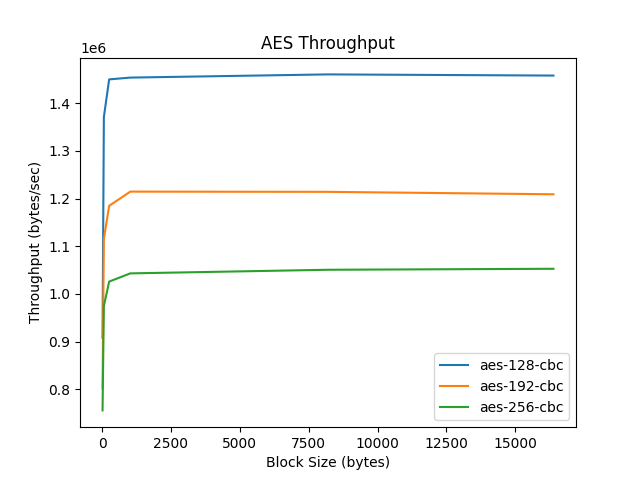
\includegraphics[width=0.5\textwidth]{./assets/aes.png}
	\caption{Throughput of AES}
	\label{fig:aes}
\end{figure}

\begin{figure}[!ht]
	\centering
	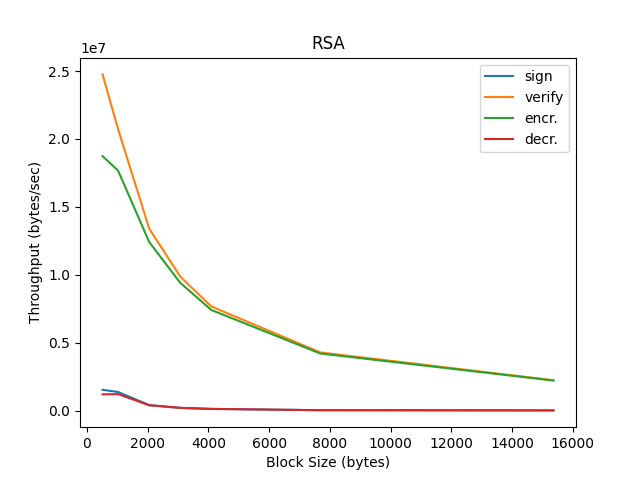
\includegraphics[width=0.5\textwidth]{./assets/rsa.png}
	\caption{Throughput of RSA}
	\label{fig:rsa}
\end{figure}

\subsubsection*{Reproduction}

Running this test is as simple as activating the venv and then running. Make sure to have openSSL version 3.3.X. This is the latest version at the time of this projects creation. 

\verb|(.venv) python task3.py|

% ============================================================================
\section*{Questions}
\subsection*{Question 1}

As mentioned before, ECB exposes patterns in the data when looking at the data as a whole; in contrast, CBC offers more obscurity, as each block that is encrypted builds on the previous. The encryption compounds in CBC, so even if the same block was encountered in the encryption process, it would be highly unlikely that they would encrypt to the same value. 

\subsection*{Question 2}

This attack is possible because of what CBC uses to try to mask the patterns that arose in the ECB encryption. The block-cipher infrastructure builds off previous encrypted blocks. If the attacker knew some sort of pattern in what the decrypted message might say, they could try to reverse engineer which bits to send through the encryption to modify the output. Authentication methods to ensure that messages have not been tampered with (such as hashing) can prevent these kinds of attacks.

\subsection*{Question 3}

Looking at the results for RSA and AES performance, we see that both protocols experienced decreased performance with increased key size, with both slowdowns appearing to be nearly linear. Overall, AES is several orders of magnitude faster than RSA.

\end{document}

